% !TEX root = ../thesis.tex

\chapter{Auswertung}
\label{ch:auswertung}

Zur Evaluation der Pipeline wurden verschiedene Teile rekonstruiert und die Ergebnisse mit vorhandenen CAD-Modellen verglichen.
Zunächst wurden mit einer Kamera am Roboterarm bereits registrierte Punktwolken aufgenommen und zusammengeführt.
Anschließend wurden mit einer fest montierten Kamera mehrere Aufnahmen eines Teils gemacht, zwischen denen dieses leicht rotiert wurde.
Abschließend wurden mit der unbeweglichen Kamera jeweils zwei Aufnahmen einer Kiste gemacht, in der sich mehrere Teile gleicher Art befanden.
Im ersten Fall waren diese räumlich gut getrennt, im zweiten Fall handelte es sich um eine volle Kiste.

Als Qualitätsmetrik wurde die Cloud-Mesh-Distanz zwischen Rekonstruktion und Ground Truth gewählt.
Dabei wird die durchschnittliche Distanz zwischen Vertices und den nächsten Faces des Vergleichobjekts betrachtet.

\begin{table}[H]
	\centering
	\begin{tabular}{| c || c | c | c | c |}
		\hline
		\textbf{Distanzen [mm]} & Rad & Zahnrad & Gehäuse & T-Stücke\\
		\hline\hline
		Fix & $0.855$ & $0.462$ & $0.364$ & $0.486$\\
		\hline
		Rotation & $0.921$ & $0.558$ & $0.751$ & $0.333$\\
		\hline
		Seg. 1 \ac{ECE} & $0.527$ & $0.318$ & $0.238$ & $0.294$\\
		\hline
		Seg. 1 \ac{RG} & $0.842$ & $0.331$ & $0.819$ & $0.316$\\
		\hline
		Seg. 1 Watershed & $0.586$ & $0.315$ & $0.756$ & $0.305$\\
		\hline
		Seg. 2 \ac{ECE} & $1.322$ & $0.393$ & $0.549$ & $0.488$\\
		\hline
		Seg. 2 \ac{RG} & $1.089$ & $0.383$ & $0.491$ & $0.326$\\
		\hline
		Seg. 2 Watershed & $0.703$ & $0.411$ & $0.701$ & $0.297$\\
		\hline
	\end{tabular}
	\caption{Cloud-Mesh-Distanzen von Rekonstruktion zu Ground Truth}
	\label{tab:dist-mesh-gt}
\end{table}

In \autoref{tab:dist-mesh-gt} sind die Distanzen von den Vertices der Rekonstruktion zu den Faces des Referenzmodells zu sehen.


\begin{table}[H]
	\centering
	\begin{tabular}{| c || c | c | c | c |}
		\hline
		\textbf{Distanzen [mm]} & Rad & Zahnrad & Gehäuse & T-Stücke\\
		\hline\hline
		Fix & $10.414$ & $2.468$ & $1.512$ & $2.398$\\
		\hline
		Rotation & $10.184$ & $2.513$ & $2.351$ & $3.224$\\
		\hline
		Seg. 1 \ac{ECE} & $11.097$ & $2.734$ & $2.692$ & $3.840$\\
		\hline
		Seg. 1 \ac{RG} & $18.414$ & $2.963$ & $5.831$ & $3.828$\\
		\hline
		Seg. 1 Watershed & $25.140$ & $7.005$ & $6.205$ & $4.449$\\
		\hline
		Seg. 2 \ac{ECE} & $19.703$ & $3.253$ & $7.711$ & $3.656$\\
		\hline
		Seg. 2 \ac{RG} & $19.744$ & $3.084$ & $4.675$ & $3.679$ \\
		\hline
		Seg. 2 Watershed & $16.056$ & $4.647$ & $3.536$ & $5.071$\\
		\hline
	\end{tabular}
	\caption{Cloud-Mesh-Distanzen von Ground Truth zu Rekonstruktion}
	\label{tab:dist-gt-mesh}
\end{table}

\begin{table}[H]
	\centering
	\begin{tabular}{| c || c | c | c | c |}
		\hline
		\textbf{Distanzverhältnis} & Rad & Zahnrad & Gehäuse & T-Stücke\\
		\hline\hline
		Fix & $0.08$ & $0.19$ & $0.24$ & $0.20$\\
		\hline
		Rotation & $0.09$ & $0.22$ & $0.32$ & $0.10$\\
		\hline
		Seg. 1 \ac{ECE} & $0.05$ & $0.12$ & $0.09$ & $0.08$\\
		\hline
		Seg. 1 \ac{RG} & $0.05$ & $0.11$ & $0.14$ & $0.08$\\
		\hline
		Seg. 1 Watershed & $0.02$ & $0.04$ & $0.12$ & $0.07$\\
		\hline
		Seg. 2 \ac{ECE} & $0.07$ & $0.12$ & $0.07$ & $0.13$\\
		\hline
		Seg. 2 \ac{RG} & $0.06$ & $0.12$ & $0.11$ & $0.09$\\
		\hline
		Seg. 2 Watershed & $0.04$ & $0.09$ & $0.20$ & $0.06$\\
		\hline
	\end{tabular}
	\caption{Verhältnis der Distanzen in \autoref{tab:dist-mesh-gt} und \autoref{tab:dist-gt-mesh}}
	\label{tab:dist-verhältnis}
\end{table}

\begin{figure}[H]
	\centering
	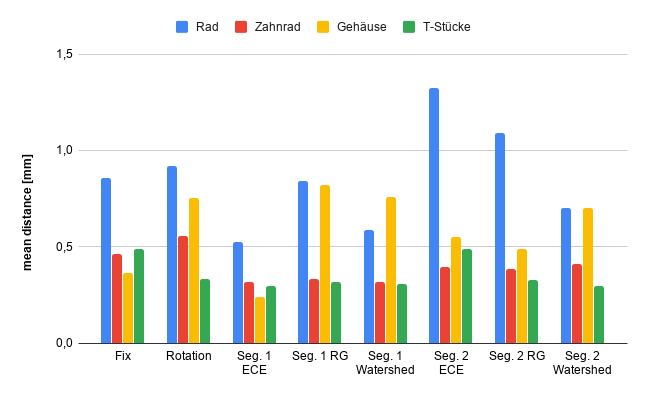
\includegraphics[width=0.49\textwidth]{images/segmentation/meanDistance1.png}
	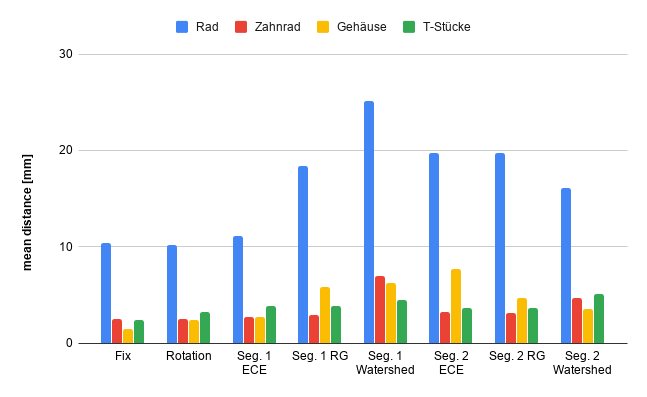
\includegraphics[width=0.49\textwidth]{images/segmentation/meanDistance2.png}
	\caption{Diagramme der Werte in \autoref{tab:dist-mesh-gt} und \autoref{tab:dist-gt-mesh}}
\end{figure}

%\begin{figure}[H]
%	\centering
%	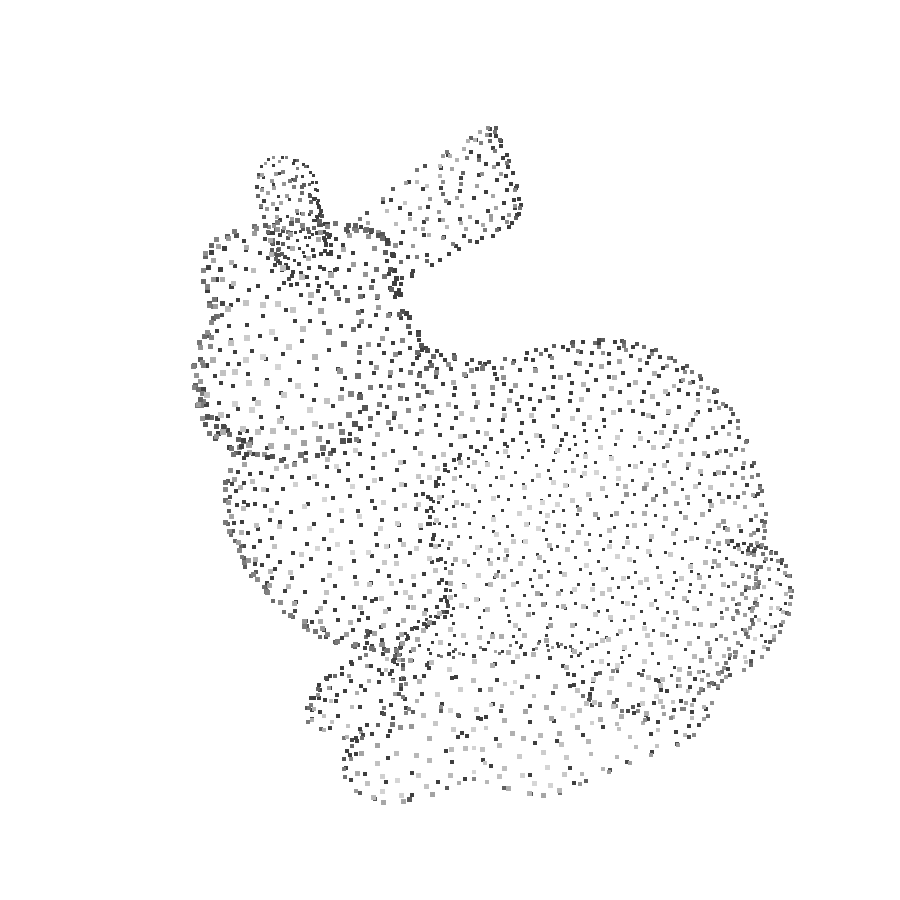
\includegraphics[width=0.33\textwidth, frame]{images/bunny_pcd.png}
%	\hspace{0.5cm}
%	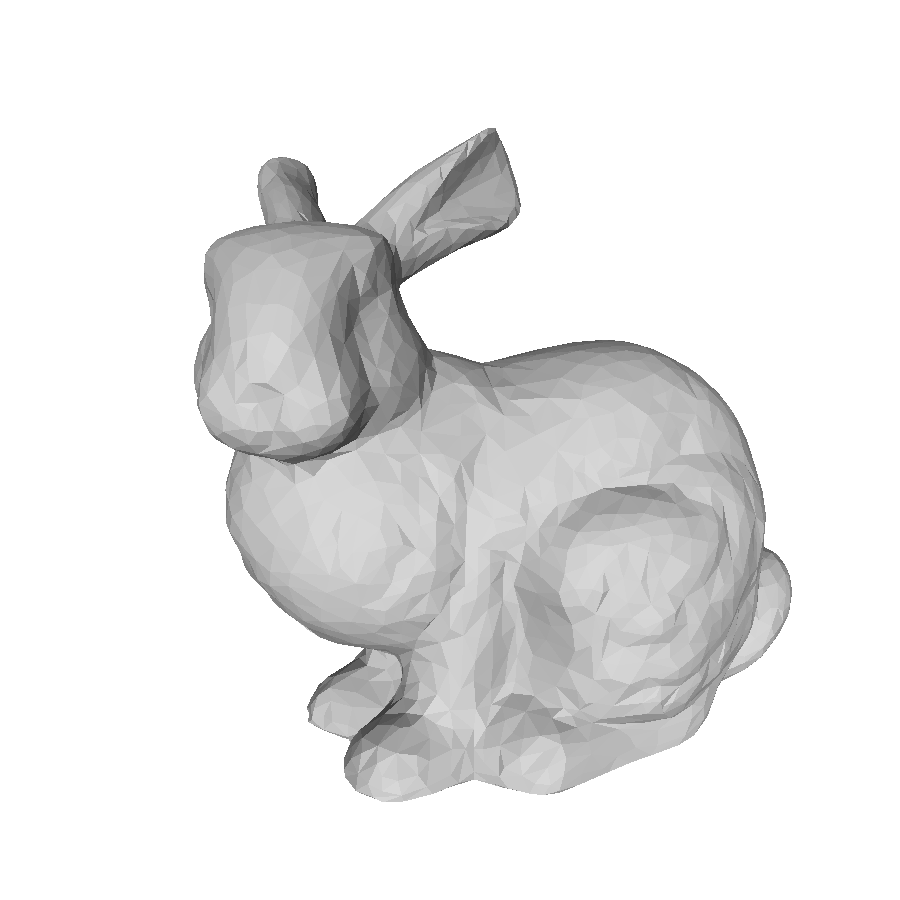
\includegraphics[width=0.33\textwidth, frame]{images/bunny_mesh.png}\\[0.5cm]
%	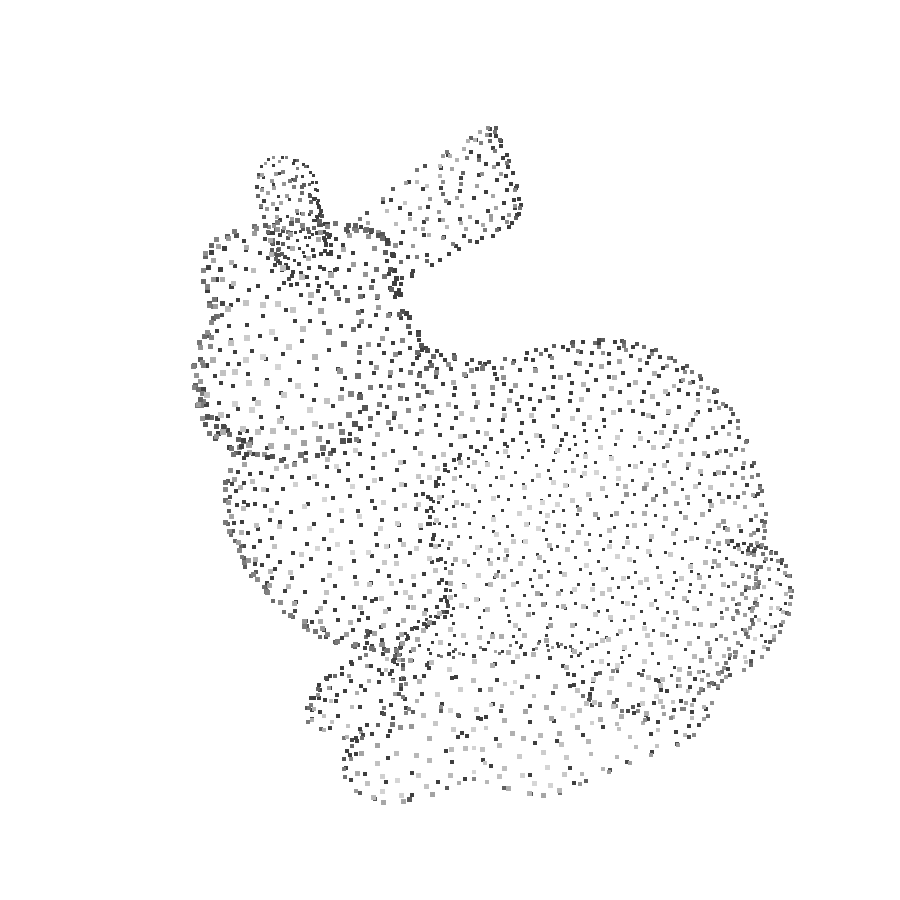
\includegraphics[width=0.33\textwidth, frame]{images/bunny_pcd.png}
%	\hspace{0.5cm}
%	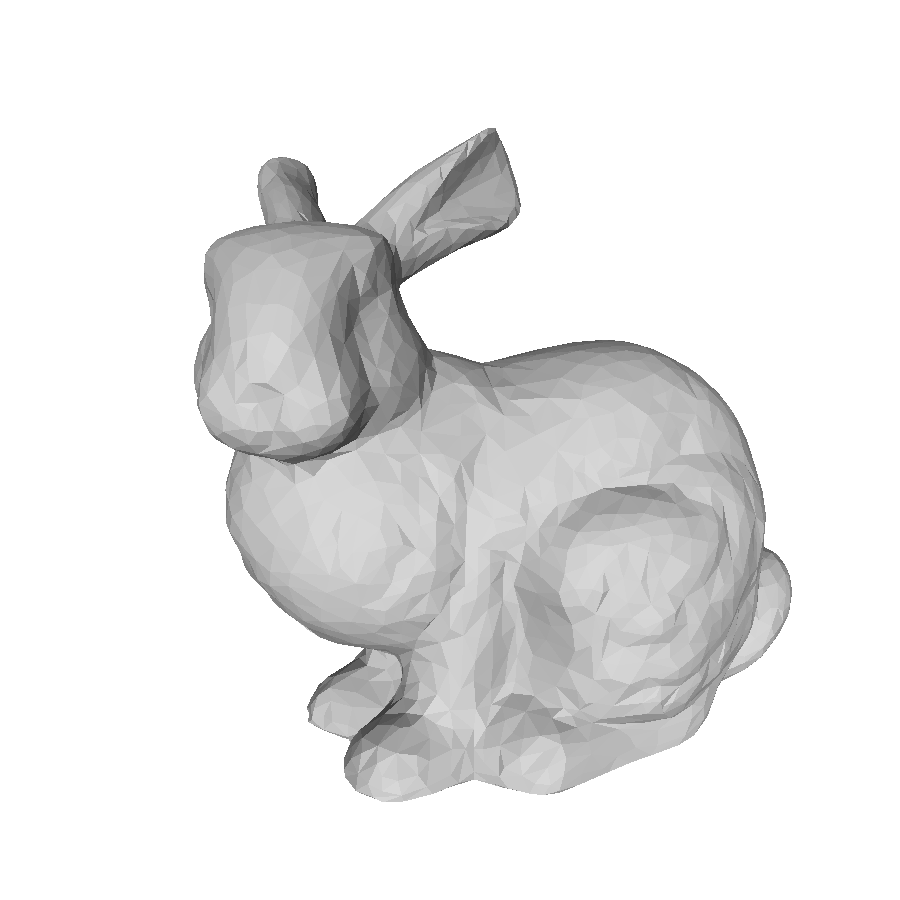
\includegraphics[width=0.33\textwidth, frame]{images/bunny_mesh.png}
%	\caption{Test image}
%	\label{fig:test}
%\end{figure}
%TODO